% !TeX program = xelatex 
\documentclass{hitreport}
\usepackage{url}
\usepackage{algorithm,float}  
\usepackage{algpseudocode}  
\usepackage{amsmath}
\usepackage{cite}
\usepackage{threeparttable}
\usepackage{subfig}
\usepackage{listings} %插入代码
\usepackage{xcolor} %代码高亮
\usepackage{tikz}
\usepackage{hyperref}



\lstset{numbers=left, %设置行号位置
	numberstyle=\tiny, %设置行号大小
	keywordstyle=\color{blue}, %设置关键字颜色
	commentstyle=\color[cmyk]{1,0,1,0}, %设置注释颜色
	frame=single, %设置边框格式
	escapeinside=``, %逃逸字符(1左面的键),用于显示中文
	breaklines, %自动折行
	extendedchars=false, %解决代码跨页时,章节标题,页眉等汉字不显示的问题
	xleftmargin=2em,xrightmargin=2em, aboveskip=1em, %设置边距
	tabsize=4, %设置tab空格数
	showspaces=false %不显示空格
}

\renewcommand{\algorithmicrequire}{\textbf{Input:}}  % Use Input in the format of Algorithm  
\renewcommand{\algorithmicensure}{\textbf{Output:}} % Use Output in the format of Algorithm  

\makeatletter
\newenvironment{breakablealgorithm}
  {% \begin{breakablealgorithm}
   \begin{center}
     \refstepcounter{algorithm}% New algorithm
     \hrule height.8pt depth0pt \kern2pt% \@fs@pre for \@fs@ruled
     \renewcommand{\caption}[2][\relax]{% Make a new \caption
       {\raggedright\textbf{\ALG@name~\thealgorithm} ##2\par}%
       \ifx\relax##1\relax % #1 is \relax
         \addcontentsline{loa}{algorithm}{\protect\numberline{\thealgorithm}##2}%
       \else % #1 is not \relax
         \addcontentsline{loa}{algorithm}{\protect\numberline{\thealgorithm}##1}%
       \fi
       \kern2pt\hrule\kern2pt
     }
  }{% \end{breakablealgorithm}
     \kern2pt\hrule\relax% \@fs@post for \@fs@ruled
   \end{center}
  }
\makeatother

% =============================================
% Part 0 Edit the info
% =============================================

\major{计算机科学与技术}
\name{孙骁}
\title{视听觉信号处理\\实验报告}
\stuid{1180300811} % 学号
\college{计算学部}
\date{2020年11月4日}
\lab{} %实验地点
\course{视听觉信号处理}
\instructor{姚鸿勋}
% \grades{}
\expname{实验一} %实验名称
% \exptype{} % 实验类型
% \partner{} % 同组学生名字
\term{2020秋季学期}

\begin{document}

\maketitle

\tableofcontents
\newpage
% =============================================
% Part 1 Header
% =============================================



% =============================================
% Part 2 Main document
% =============================================

\section{实验目标和内容}

\subsection{实验目标}
\begin{enumerate}
\item 掌握图像处理中常见的空域滤波算法;
\item 掌握图像处理中常见的边缘检测算子.
\end{enumerate}

\subsection{实验内容}
\begin{enumerate}
\item \label{item:1}实现给图像添加高斯噪声和椒盐噪声,显示并保存结果图像;
\item 实现图像中的空域滤波:中值滤波和均值滤波算法,选取合适的方法对\ref{item:1}中的图像进行平滑处理,显示并保存结果图像;
\item 实现图像中的边缘检测算子:Canny算子和 Sobel算子;
\item 自己学习新算法,简述算法原理. 显示并保存实验结果。与对比方法形成优缺点说明.
\end{enumerate}

\section{实验环境}

\begin{enumerate}
\item Anaconda 4.8.4
\item Python 3.7.4
\item PyCharm 2019.1 (Professional Edition)
\item Windows 10 2004
\end{enumerate}

\section{实验原理}

\subsection{空域滤波算法}

空间滤波是通过把每个像素值替换为该像素及其邻域像素的函数值来修改图像的一种方法。如果对于图像像素执行的运算是线性的,则称该滤波器为线性空间滤波器;否则称该滤波器为非线性空间滤波器。下面主要介绍线性滤波器。

线性空间滤波器在图像\textit{f}和滤波器核\textit{w}之间执行乘积之和运算。对于图像\textit{f}、卷积核\textit{w}与输出图像\textit{g},在图像任意一点$\left(x,y\right)$处,滤波器的响应$g\left(x,y\right)$是核系数和核所覆盖的图像像素的乘积之和。对于大小为$m\times n$的核,假设$m=2a+1$和$n=2b+1$,其中\textit{a}和\textit{b}是非负整数。一般来说,大小为$m\times n$的核对大小为$M\times N$的图像的线性空间滤波可以表示为
\begin{align}
g\left(x,y\right) = \sum_{s=-a}^{a}\sum_{t=-b}^{b}w\left(s,t\right)f\left(x+s,y+t\right),
\end{align}
式中\textit{x}和\textit{y}发生变化,使得核的中心(原点)能够访问\textit{f}中的每个像素。

\subsubsection{中值滤波算法}

中值滤波并不是线性的滤波算法,中值滤波会将待滤波图像的相应位置的像素值替换为滤波核模板覆盖的像素的中值,假如我们使用$3\times3$的滤波核,则滤波后的图像可以表示为:
\begin{align}
\begin{split}
g\left(x,y\right) = \text{mid}\{&f\left(x-1,y-1\right),f\left(x,y-1\right),f\left(x+1,y-1\right),\\
&f\left(x-1,y\right),\;\;\;\;\;\;f\left(x,y\right),\;\;\;\;\;\;f\left(x+1,y\right),\\
&f\left(x+1,y-1\right),f\left(x+1,y\right),f\left(x+1,y+1\right)\}
\end{split}
\end{align}

中值滤波抑制随机点状噪声的效果良好,但是随着窗口的扩大,有效信号的损失也将明显增大。本次实验选择的窗口为$3\times3$的。

\subsubsection{均值滤波算法}

均值滤波是一种线性滤波算法,均值滤波有取阈值的邻域平均法、邻域加权平均法以及等加权平均法。实验中实现的是等加权平均法,采用$3\times 3$的滤波核,滤波后的图像可以表示为:
\begin{align}
g\left(x,y\right) = \sum_{i=-m}^{m}\sum_{j=-n}^{n}w\left(i,j\right)f\left(x-i,y-j\right),
\end{align}
其中,$w$为权值矩阵,为
\begin{align}
w=\frac{1}{9}\left( \begin{matrix}
	1&		1&		1\\
	1&		1&		1\\
	1&		1&		1\\
\end{matrix} \right).
\end{align}

\subsection{边缘检测算法}

基于边缘检测的分析不易受整体光照强度变化的影响,许多图像理解方法都以边缘为基础。边缘检测强调的是图像对比度。检测对比度即亮度上的差别,可以增强图像中的边界特征,这些边界出现正是图像亮度上的差别。目标边界实际上是亮度级的阶梯变化,而边缘是阶梯变化的位置。可以使用一阶微分使边缘变化增强检测边缘位置,除当输入扫信号没有发生变化。

亮度变化可能通过对相邻点进行差分处理来增强。对水平方向上的相邻点进行差分处于是可以检测垂直方向上的亮度变化,通常被称为水平边缘检测算子(horizontal edge detector)。因为其差分值为零,所以水平算子寻不会显示水平方向的亮度变化。同时,需要一个垂直边缘检测算子(vertical edge detector)对垂直方向上的相邻点进行差分处理,这样可以确定水平方向上,而不是垂直方向上的亮度变化,因而垂直边缘检测算子检测的是水平边缘。组合两种算子处理之后的结果即可得到图像的边缘检测结果。

\subsubsection{Sobel边缘检测算法}

在图像处理中,Sobel算子的这个通用形式缩合了一条坐标轴上最优平滑和另一条坐标轴上的最优差分。换而言之,Sobel 算子有两个,一个是检测水平边缘的 ;另一个是检测垂直边缘的 。它对于像素的位置的影响做了加权,可以降低边缘模糊程度,因此效果更好。由于Sobel算子是滤波算子的形式,用于提取边缘,可以利用快速卷积函数, 简单有效,因此应用广泛。但缺点就是Sobel算子并没有将图像的主体与背景严格地区分开来,即:Sobel算子没有基于图像灰度进行处理,由于Sobel算子没有严格地模拟人的视觉生理特征,所以提取的图像轮廓有时并不能令人满意。

利用Sobel算子进行边缘检测的程序见附录\ref{app:sobel}。


\subsubsection{Canny边缘检测算法}

Canny缘检测算法是公认的性能最为优良的边缘检测算法之一。Canny算法不是像Roberts、Prewitt、Sobel等这样简单梯度算子或锐化模板,它是在梯度算子基础上,引入了一种能获得抗噪性能好、定位精度高的单像素边缘的计算策略。

Canny边缘检测算法主要分为四个步骤:
\begin{enumerate}
\item 利用高斯滤波器对原始图像进行平滑滤波,以提高算法的抗噪性;
\item 用一阶有限差分近似代替偏导数,计算图像梯度强度和方向。计算梯度可以利用Roberts、 Prewitt、Sobel等算子;\label{sec:2}
\item 利用第\ref{sec:2}步梯度方向划分进行梯度强度的非极大抑制,获取单像素边缘点;
\item 双阈值进行边缘的二值化。
\end{enumerate}

利用Sobel算子进行边缘检测的程序见附录\ref{app:canny}。



\subsection{Laplacian锐化}

拉普拉斯锐化图像是根据图像某个像素的周围像素到此像素的突变程度有关,也就是说它的依据是图像像素的变化程度。我们知道,一个函数的一阶微分描述了函数图像是朝哪里变化的,即增长或者降低;而二阶微分描述的则是图像变化的速度,急剧增长下降还是平缓的增长下降。那么据此我们可以猜测出依据二阶微分能够找到图像的色素的过渡程度,例如白色到黑色的过渡就是比较急剧的。

换言之:当邻域中心像素灰度低于它所在的领域内其它像素的平均灰度时,此中心像素的灰度应被进一步降低,当邻域中心像素灰度高于它所在的邻域内其它像素的平均灰度时,此中心像素的灰度应被进一步提高,以此实现图像的锐化处理。

拉普拉斯锐化的模板矩阵有两种,分别为四邻域模板和八邻域模板,如下:

\begin{align}
L_4=\left( \begin{matrix}
	0&		-1&		0\\
	-1&		4&		-1\\
	0&		-1&		0\\
\end{matrix} \right)\qquad L_8=\left( \begin{matrix}
	-1&		-1&		-1\\
	-1&		8&		-1\\
	-1&		-1&		-1\\
\end{matrix} \right)
\end{align}

\section{实验步骤}

实验中所有代码在附录可见。

\subsection{图像添加椒盐噪声和高斯噪声}\label{sec:noise}

为图像添加高斯噪声的函数如下:
\begin{lstlisting}[language=python]
def add_gauss_noise(img, mean, variance):
    img = np.array(img / 255, dtype=float)
    noise = np.random.normal(mean, variance ** 0.5, img.shape)
    out = img + noise
    out = np.clip(out, 0.0, 1.0)
    out = np.uint8(out * 255)
    return out
\end{lstlisting}

为图像添加椒盐噪声的函数如下:
\begin{lstlisting}[language=python]
def add_salt_pepper_noise(img, proportion):
    length, width = img.shape[0], img.shape[1]
    out = img
    noise_number = int(length * width * proportion)
    print(noise_number)
    for i in range(noise_number):
        x = np.random.randint(0, length)
        y = np.random.randint(0, width)
        if np.random.randint(0, 2) == 0:
            out[x, y] = 0
        else:
            out[y, x] = 255
    return out
\end{lstlisting}
其中参数proportion控制生成噪声生成比例。

\subsection{中值滤波算法}\label{sec:median}

对灰度图像的中值滤波算法如下:
\begin{lstlisting}[language=python]
def median_filter_gray(img_matrix):
    img_filter = img_matrix.copy()
    height, width = np.shape(img_filter)
    # kernel = np.ones((3, 3))
    height_top = height - 1
    width_top = width - 1
    for i in range(1, height_top):
        for j in range(1, width_top):
            img_filter[i, j] = np.median(img_filter[i - 1:i + 2, j - 1:j + 2].copy().reshape((1, -1))[0])
    img_filter = img_filter[1:height_top, 1:width_top]
    return img_filter
\end{lstlisting}

\subsection{均值滤波算法}\label{sec:mean}

对灰度图像的均值滤波算法如下:
\begin{lstlisting}[language=python]
def mean_filter_gray(img_matrix):
    img_filter = img_matrix.copy()
    height, width = np.shape(img_filter)
    kernel = np.ones((3, 3))
    height_top = height - 1
    width_top = width - 1
    for i in range(1, height_top):
        for j in range(1, width_top):
            img_filter[i, j] = np.sum(kernel * img_filter[i - 1:i + 2, j - 1:j + 2]) // (3 ** 2)
    img_filter = img_filter[1:height_top, 1:width_top]
    return img_filter
\end{lstlisting}

\subsection{Sobel算子边缘检测}\label{sec:sobel}

Sobel算子边缘检测算法如下:
\begin{lstlisting}[language=python]
def sobel_detection_gray(img_matrix):
    print("start to detection the edge of gray image with sobel operator")
    img_sobel = img_matrix.copy()
    height, width = np.shape(img_sobel)
    # print(np.shape(img_sobel))
    sobel_operator_x = np.array([[-1, 0, 1], [-2, 0, 2], [-1, 0, 1]])
    sobel_operator_y = np.array([[1, 2, 1], [0, 0, 0], [-1, -2, -1]])
    new_img = np.zeros((height, width))
    height_top = height - 1
    width_top = width - 1
    for i in range(1, height_top):
       for j in range(1, width_top):
           new_x = abs(np.sum(img_sobel[i - 1:i + 2, j - 1:j + 2] * sobel_operator_x))
           new_y = abs(np.sum(img_sobel[i - 1:i + 2, j - 1:j + 2] * sobel_operator_y))
           new_img[i, j] = np.sqrt(np.square(new_x) + np.square(new_y))
    new_img = new_img[1:height_top, 1:width_top]
    print("finish detecting the edge of gray image with sobel operator")
    return np.uint8(new_img)
\end{lstlisting}

\subsection{Canny算子边缘检测}\label{sec:canny}

Canny边缘检测的算法如下,其中Canny边缘检测的四个步骤依次拆分为四个函数,有相应的注释。
\begin{lstlisting}[language=python]
class CannyEdgeDetection(object):
    """
    Canny边缘检测
    """
    def __init__(self):
        # self.img_rgb = read_source_img_from_file()
        self.img_gray = read_source_img_with_gray_from_file()
        self.img_matrix = np.asarray(self.img_gray)
        self.img_matrix_filter = np.pad(self.img_matrix, ((2, 2), (2, 2)), 'constant', constant_values=(0, 0))
        self.gaussian_filter = None
        self.img_gradient = None
        self.theta = None
        self.matrix_y = np.array([[-1, 0, 1], [-1, 0, 1], [-1, 0, 1]])
        self.matrix_x = np.array([[-1, -1, -1], [0, 0, 0], [1, 1, 1]])
        self.nms_result = None
        self.dtd_result = None

    def gaussian_filtering(self):
        """
        高斯平滑
        :return: 无
        """
        print("start to gauss filter of the image")
        sigma1 = sigma2 = 1
        sum = 0
        gaussian = np.zeros([5, 5])
        for i in range(5):
            for j in range(5):
                gaussian[i, j] = np.exp(
                    -1 / 2 * (np.square(i - 3) / np.square(sigma1) + (np.square(j - 3) / np.square(sigma2)))) / (
                                         2 * np.pi * sigma1 * sigma2)
                sum = sum + gaussian[i, j]
        gaussian = gaussian / sum
        # print(gaussian)

        img_gauss = self.img_matrix_filter.copy()
        height, width = np.shape(img_gauss)
        new_img = np.zeros((height, width))
        height_top = height - 2
        width_top = width - 2
        for i in range(2, height_top):
            for j in range(2, width_top):
                new_img[i, j] = np.sum(gaussian * img_gauss[i - 2:i + 3, j - 2:j + 3])
        # print(np.shape(new_img))
        new_img = new_img[1:height_top + 1, 1:width_top + 1]
        # print(np.shape(new_img))
        self.gaussian_filter = new_img
        print("finish gauss filtering the image")
        show_img(np.uint8(new_img), "gauss filtering the image")
        # return np.uint8(new_img)

    def calculate_gradient_and_direction(self):
        """
        计算各像素的梯度和梯度方向
        :return: 无
        """
        print("start to calculate the gradient and direction of the image")
        height, width = np.shape(self.gaussian_filter)
        # print(np.shape(self.gaussian_filter))
        img_gradient = self.gaussian_filter.copy()
        self.img_gradient = np.zeros((height, width), dtype="uint8")
        self.theta = np.zeros((height, width))
        height_top = height - 1
        width_top = width - 1
        for i in range(1, height_top):
            for j in range(1, width_top):
                gradient_y = (
                    np.dot(np.array([1, 1, 1]), (self.matrix_y * img_gradient[i - 1:i + 2, j - 1:j + 2]))).dot(
                    np.array([[1], [1], [1]]))
                gradient_x = (
                    np.dot(np.array([1, 1, 1]), (self.matrix_x * img_gradient[i - 1:i + 2, j - 1:j + 2]))).dot(
                    np.array([[1], [1], [1]]))

                if gradient_x[0] == 0:
                    self.theta[i - 1, j - 1] = 90
                    continue
                else:
                    temp_direction = (np.arctan(gradient_y[0] / gradient_x[0])) * 180 / np.pi
                if gradient_x[0] * gradient_y[0] > 0:
                    if gradient_x[0] > 0:
                        self.theta[i - 1, j - 1] = np.abs(temp_direction)
                    else:
                        self.theta[i - 1, j - 1] = np.abs(temp_direction) - 180
                if gradient_x[0] * gradient_y[0] < 0:
                    if gradient_x[0] > 0:
                        self.theta[i - 1, j - 1] = -1 * np.abs(temp_direction)
                    else:
                        self.theta[i - 1, j - 1] = 180 - np.abs(temp_direction)
                self.img_gradient[i, j] = np.sqrt(np.square(gradient_x) + np.square(gradient_y))

        for i in range(1, height_top):
            for j in range(1, width_top):
                if ((self.theta[i, j] >= -22.5) and (self.theta[i, j] < 22.5)) or (
                        (self.theta[i, j] <= -157.5) and (self.theta[i, j] >= -180)) or (
                        (self.theta[i, j] >= 157.5) and (self.theta[i, j] < 180)):
                    self.theta[i, j] = 0.0
                elif ((self.theta[i, j] >= 22.5) and (self.theta[i, j] < 67.5)) or (
                        (self.theta[i, j] <= -112.5) and (self.theta[i, j] >= -157.5)):
                    self.theta[i, j] = 45.0
                elif ((self.theta[i, j] >= 67.5) and (self.theta[i, j] < 112.5)) or (
                        (self.theta[i, j] <= -67.5) and (self.theta[i, j] >= -112.5)):
                    self.theta[i, j] = 90.0
                elif ((self.theta[i, j] >= 112.5) and (self.theta[i, j] < 157.5)) or (
                        (self.theta[i, j] <= -22.5) and (self.theta[i, j] >= -67.5)):
                    self.theta[i, j] = -45.0
        show_img(self.img_gradient, "calculate the gradient and direction of the image")
        print("finish calculating the gradient and direction of the image")

    def non_maximum_suppression(self):
        """
        非极大值抑制
        :return: 无
        """
        print("start to nms")
        height, width = np.shape(self.img_gradient)
        img = self.img_gradient.copy()
        img_nms = np.zeros((height, width))
        height_top = height - 1
        width_top = width - 1
        for i in range(1, height_top):
            for j in range(1, width_top):
                if (self.theta[i, j] == 0.0) and (img[i, j] == np.max([img[i, j], img[i + 1, j], img[i - 1, j]])):
                    img_nms[i, j] = img[i, j]
                if (self.theta[i, j] == 45.0) and (
                        img[i, j] == np.max([img[i, j], img[i - 1, j + 1], img[i + 1, j - 1]])):
                    img_nms[i, j] = img[i, j]
                if (self.theta[i, j] == 90.0) and (img[i, j] == np.max([img[i, j], img[i, j + 1], img[i, j - 1]])):
                    img_nms[i, j] = img[i, j]
                if (self.theta[i, j] == -45.0) and (
                        img[i, j] == np.max([img[i, j], img[i - 1, j - 1], img[i + 1, j + 1]])):
                    img_nms[i, j] = img[i, j]
        self.nms_result = img_nms
        show_img(self.nms_result, "nms result")
        print("finish nms")

    def dual_threshold_detection(self):
        """
        双阈值检测
        :return: 无
        """
        print("start to dual threshold detection")
        dtd_img = np.zeros(np.shape(self.nms_result))
        TL = 0.15 * np.max(self.nms_result)
        TH = 0.3 * np.max(self.nms_result)
        nms = self.nms_result
        height, width = np.shape(self.nms_result)
        height_top = height - 1
        width_top = width - 1
        for i in range(1, height_top):
            for j in range(1, width_top):
                if nms[i, j] < TL:
                    dtd_img[i, j] = 0
                elif nms[i, j] > TH:
                    dtd_img[i, j] = 255
                elif (nms[i + 1, j] < TH) or (nms[i - 1, j] < TH) or (nms[i, j + 1] < TH) or (nms[i, j - 1] < TH) or (
                        nms[i - 1, j - 1] < TH) or (nms[i - 1, j + 1] < TH) or (nms[i + 1, j + 1] < TH) or (
                        nms[i + 1, j - 1] < TH):
                    dtd_img[i, j] = 255
        self.dtd_result = dtd_img
        show_img(self.dtd_result, "dual threshold detection")
        print("finish dual threshold detection")

    def canny_detection_gray(self):
        """
        Canny检测类的主程序
        :return:
        """
        print("start to detect the edge of image with canny operator")
        self.gaussian_filtering()
        self.calculate_gradient_and_direction()
        self.non_maximum_suppression()
        self.dual_threshold_detection()
        print("finish detecting the edge of image with canny operator")


\end{lstlisting}

\subsection{拉普拉斯锐化算法}\label{sec:lap}

拉普拉斯锐化算法函数如下:
\begin{lstlisting}[language=python]
class LaplacianSharpening(object):
    def __init__(self):
        self.img = read_source_img_with_gray_from_file()
        self.img_matrix = np.asarray(self.img)
        self.img_matrix_filter = np.pad(self.img_matrix, ((1, 1), (1, 1)), 'constant', constant_values=(0, 0))
        self.laplace_4 = np.array([[0, -1, 0], [-1, 5, -1], [0, -1, 0]])
        self.laplace_8 = np.array([[-1, -1, -1], [-1, 9, -1], [-1, -1, -1]])

    def laplacian_sharpening(self):
        print("start laplace sharpen")
        img_matrix = self.img_matrix_filter.copy()
        height, width = np.shape(img_matrix)
        height_top = height - 1
        width_top = width - 1
        laplace_4_img = np.zeros((height, width))
        laplace_8_img = np.zeros((height, width))
        for i in range(1, height_top):
            for j in range(1, width_top):
                laplace_4_img[i, j] = np.sum(self.laplace_4 * img_matrix[i - 1:i + 2, j - 1:j + 2])
                laplace_8_img[i, j] = np.sum(self.laplace_8 * img_matrix[i - 1:i + 2, j - 1:j + 2])
                if laplace_4_img[i, j] <= 0:
                    laplace_4_img[i, j] = 0
                if laplace_8_img[i, j] <= 0:
                    laplace_8_img[i, j] = 0
        laplace_4_img = laplace_4_img[1:height_top, 1:width_top]
        laplace_8_img = laplace_8_img[1:height_top, 1:width_top]
        print("finish laplace sharpen")
        return np.uint8(laplace_4_img), np.uint8(laplace_8_img)
\end{lstlisting}

\section{实验结果}

实验测试选用lena图像,原图及灰度图如图(\ref{fig:lena})所示。

\begin{figure}[h]
	\centering
	\subfloat[lena彩色图]{
		\label{fig:lenacolor}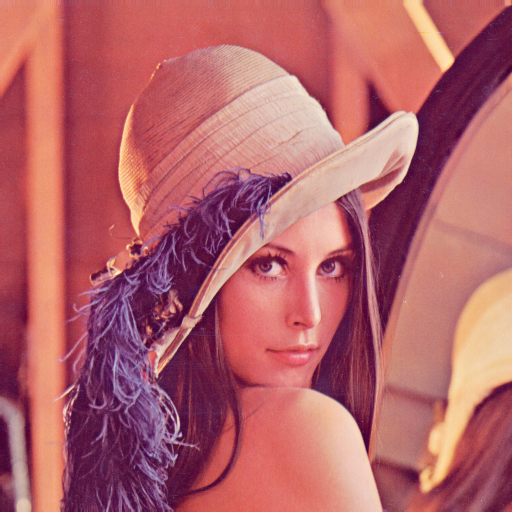
\includegraphics[width=.4\textwidth]{lena.png}}\hspace{20pt}
	\subfloat[lena灰度图]{
		\label{fig:lenagray}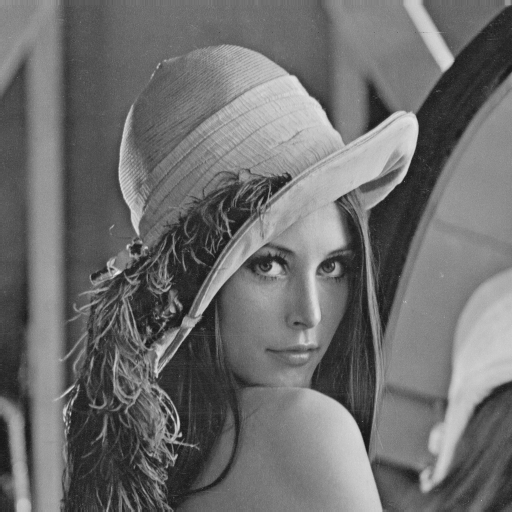
\includegraphics[width=.4\textwidth]{graylena.png}}
	\caption{lena 彩色图与灰度图}\label{fig:lena}
\end{figure}

\subsection{图像添加椒盐噪声和高斯噪声}

给lena彩色图像添加椒盐噪声的结果如图(\ref{fig:lenasalt})所示,添加高斯噪声的结果如图(\ref{fig:lenagauss})所示。

\begin{figure}[htb]
	\centering
	\subfloat[lena彩色图添加椒盐噪声]{
		\label{fig:lenasalt}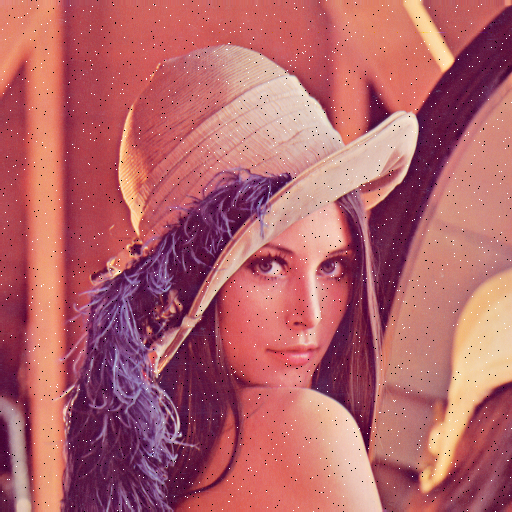
\includegraphics[width=.4\textwidth]{addsaltpeppernoise.png}}\hspace{20pt}
	\subfloat[lena彩色图添加高斯噪声]{
		\label{fig:lenagauss}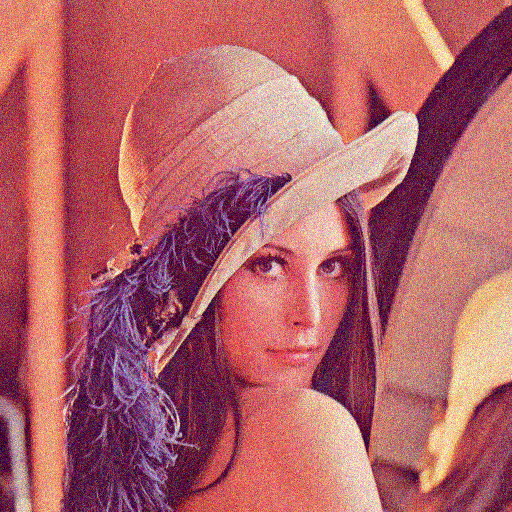
\includegraphics[width=.4\textwidth]{addgaussnoise.png}}
	\caption{lena 图像添加椒盐噪声和高斯噪声}\label{fig:lenanoise}
\end{figure}

\subsection{对添加噪声的图像进行中值滤波}

对添加椒盐噪声和高斯噪声的lena图片使用章节\ref{sec:median}算法分别进行中值滤波,结果如图(\ref{fig:lenamedian})所示。

\begin{figure}[htb]
	\centering
	\subfloat[lena彩色图椒盐噪声中值滤波]{
		\label{fig:lenasaltmedian}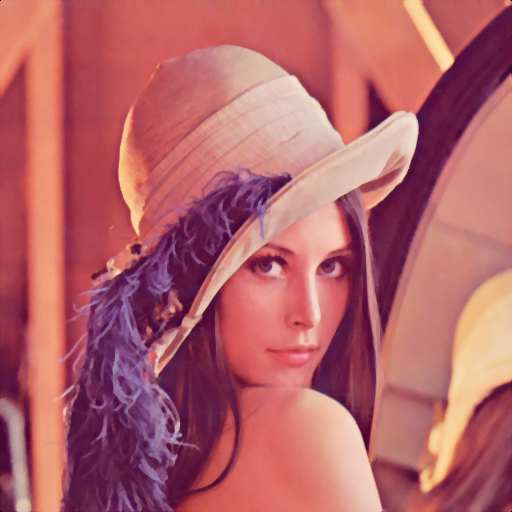
\includegraphics[width=.4\textwidth]{medianfilterofsaltpeppernoise.png}}\hspace{20pt}
	\subfloat[lena彩色图高斯噪声中值滤波]{
		\label{fig:lenagaussmedian}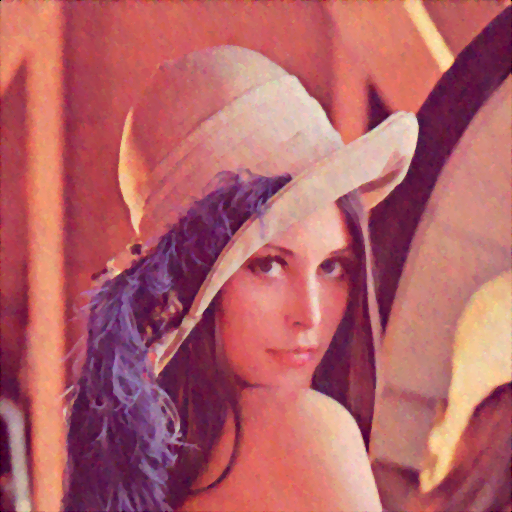
\includegraphics[width=.4\textwidth]{medianfilterofgaussnoise.png}}
	\caption{lena 图像椒盐噪声和高斯噪声进行中值滤波}\label{fig:lenamedian}
\end{figure}

\subsection{对添加噪声的图像进行均值滤波}

对添加椒盐噪声和高斯噪声的lena图片使用章节\ref{sec:mean}算法分别进行均值滤波,结果如图(\ref{fig:lenamean})所示。

\begin{figure}[htb]
	\centering
	\subfloat[lena彩色图椒盐噪声均值滤波]{
		\label{fig:lenasaltmean}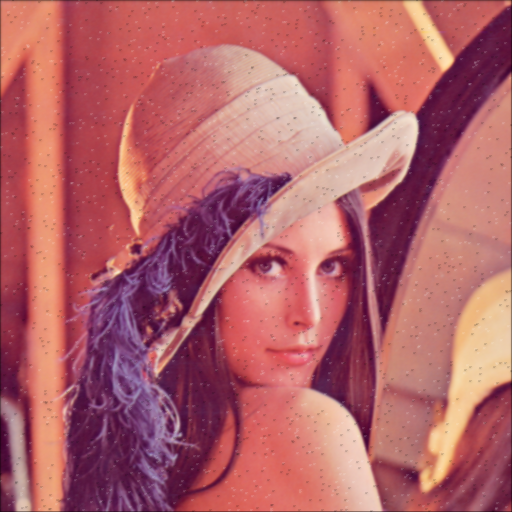
\includegraphics[width=.4\textwidth]{meanfilterofsaltpeppernoise.png}}\hspace{20pt}
	\subfloat[lena彩色图高斯噪声均值滤波]{
		\label{fig:lenagaussmean}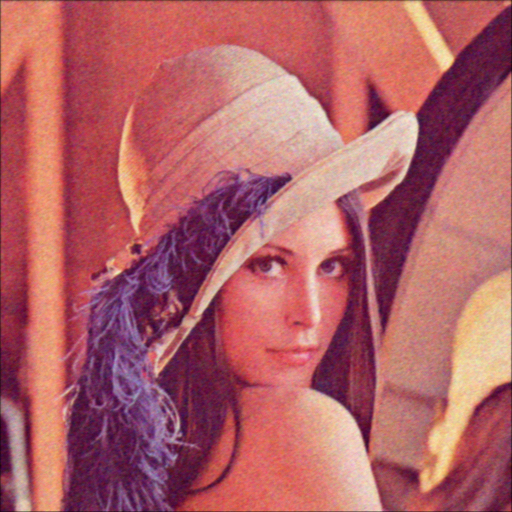
\includegraphics[width=.4\textwidth]{meanfilterofgaussnoise.png}}
	\caption{lena 图像椒盐噪声和高斯噪声进行均值滤波}\label{fig:lenamean}
\end{figure}


\subsection{Sobel算子边缘检测结果}

对lena灰度图使用章节\ref{sec:sobel}的算法进行Sobel算子边缘检测,得到的结果如图(\ref{fig:lenasobel})所示。

\begin{figure}[htb]
	\centering
	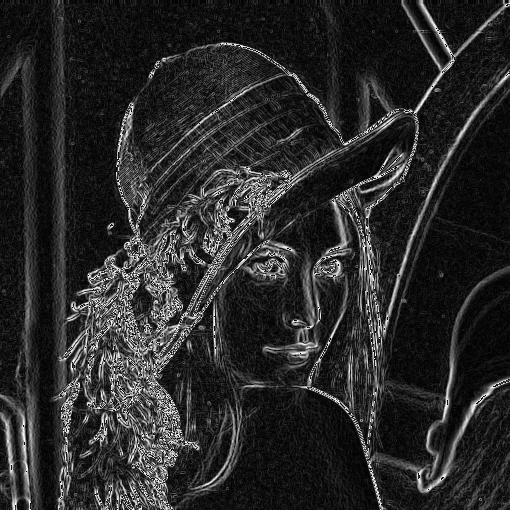
\includegraphics[width=0.4\linewidth]{sobeldetectionofgarylena.png}
	\caption{对lena灰度图进行Sobel边缘检测}\label{fig:lenasobel}
\end{figure}

\subsection{Canny算子边缘检测结果}

对lena灰度图使用章节\ref{sec:canny}的算法进行Canny算子边缘检测,得到的结果如图(\ref{fig:lenacanny})所示。

\begin{figure}[htb]
	\centering
	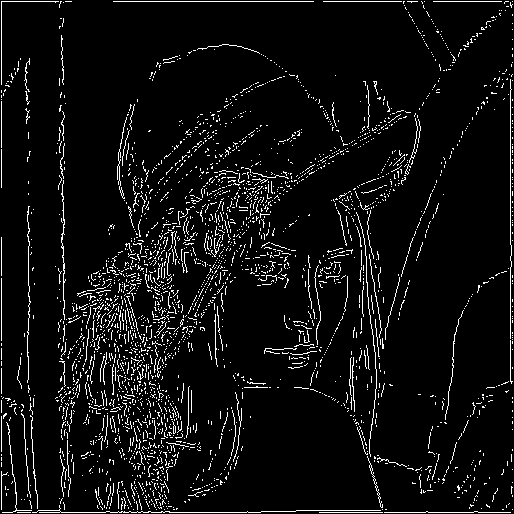
\includegraphics[width=0.4\linewidth]{cannyedgedetectionoflena.png}
	\caption{对lena灰度图进行Canny边缘检测}\label{fig:lenacanny}
\end{figure}

\subsection{拉普拉斯锐化}

对lena灰度图使用章节\ref{sec:lap}的四邻域模板和八邻域模板进行拉普拉斯锐化,得到的结果如图(\ref{fig:lap})所示。

\begin{figure}[htb]
	\centering
	\subfloat[lena灰度图使用四邻域模板拉普拉斯锐化]{
		\label{fig:lap4}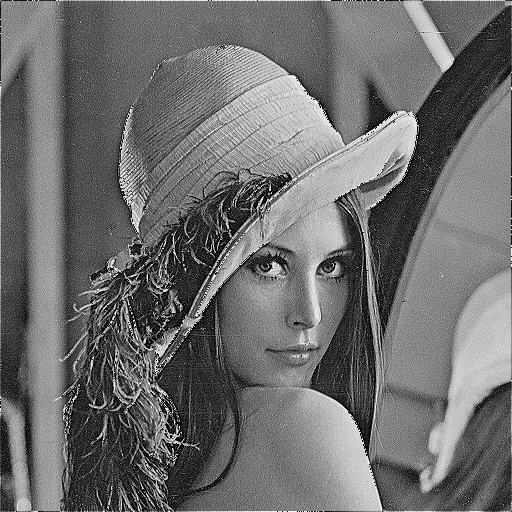
\includegraphics[width=.4\textwidth]{laplacesharpeningwith4area.png}}\hspace{20pt}
	\subfloat[lena灰度图使用八邻域模板拉普拉斯锐化]{
		\label{fig:lap8}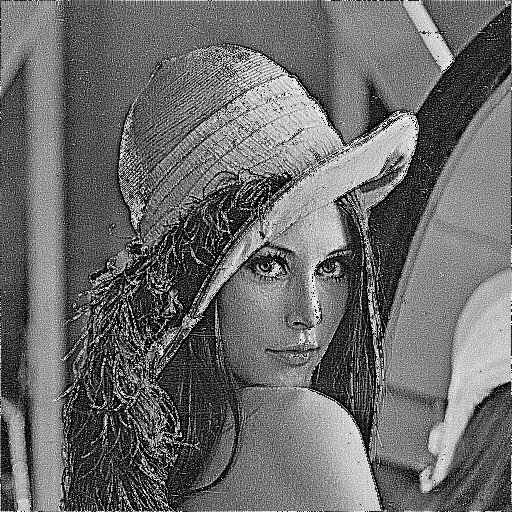
\includegraphics[width=.4\textwidth]{laplacesharpeningwith8area.png}}
	\caption{lena 灰度图像的拉普拉斯锐化结果}\label{fig:lap}
\end{figure}


\section{实验结论}

\begin{enumerate}
\item 为彩色图添加噪声时需要将彩色图的像素值先进行归一化,再添加噪声;
\item 中值滤波对椒盐噪声的去噪效果较好,均值滤波对高斯噪声的去噪效果较好;
\item 基于Sobel算子的边缘检测算法对图像的边缘检测效果不如基于Canny算子的边缘检测算法效果好;
\item 拉普拉斯锐化的效果中,使用八邻域模板的效果较四邻域模板的效果会凸显更多的细节,边缘更加“锐利”。
\end{enumerate}

\renewcommand\refname{参考文献}
 
\begin{thebibliography}{1}
\bibitem{book:li}
Rafael C. Gonzalez \& Richard E. Woods (2020). Digital Image Processing (4th ed.).

\end{thebibliography}

\newpage
\begin{appendices}\label{sec:app}

\section{lena图像添加噪声--add\_gauss\_salt\_pepper\_noise.py}\label{app:niose}
\begin{lstlisting}[language=python]
import numpy as np
from src.read_write_img import *


def add_noise():
    img = read_source_img_from_file()
    gauss_noise_img = add_gauss_noise(img, 0, 0.01)
    write_img_to_file(gauss_noise_img, 'add gauss noise')
    show_img(gauss_noise_img, 'add gauss noise')
    salt_pepper_noise_img = add_salt_pepper_noise(img, 0.01)
    write_img_to_file(salt_pepper_noise_img, 'add salt pepper noise')
    show_img(salt_pepper_noise_img, 'add salt pepper noise')


def add_gauss_noise(img, mean, variance):
    img = np.array(img / 255, dtype=float)
    noise = np.random.normal(mean, variance ** 0.5, img.shape)
    out = img + noise
    out = np.clip(out, 0.0, 1.0)
    out = np.uint8(out * 255)
    return out


def add_salt_pepper_noise(img, proportion):
    length, width = img.shape[0], img.shape[1]
    out = img
    noise_number = int(length * width * proportion)
    print(noise_number)
    for i in range(noise_number):
        x = np.random.randint(0, length)
        y = np.random.randint(0, width)
        if np.random.randint(0, 2) == 0:
            out[x, y] = 0
        else:
            out[y, x] = 255
    return out


if __name__ == '__main__':
    add_noise()

\end{lstlisting}

\section{中值滤波和均值滤波算法--filter\_img.py}
\begin{lstlisting}[language=python]
import numpy as np
from PIL import Image
from src.read_write_img import *


class FilterImg(object):

    def __init__(self, img):
        self.img = img
        self.img_matrix = np.asarray(self.img)
        # self.img_filter = np.pad(self.img_matrix, ((2, 2), (2, 2)), 'constant', constant_values=(0, 0))
        self.b, self.g, self.r = cv.split(self.img)
        self.b_matrix = np.asarray(self.b)
        self.g_matrix = np.asarray(self.g)
        self.r_matrix = np.asarray(self.r)
        self.b_matrix_filter = np.pad(self.b_matrix, ((1, 1), (1, 1)), 'constant', constant_values=(0, 0))
        self.g_matrix_filter = np.pad(self.g_matrix, ((1, 1), (1, 1)), 'constant', constant_values=(0, 0))
        self.r_matrix_filter = np.pad(self.r_matrix, ((1, 1), (1, 1)), 'constant', constant_values=(0, 0))

    def filter_img(self):
        self.median_filter_rgb()
        self.mean_filter_rgb()

    @staticmethod
    def median_filter_gray(img_matrix):
        img_filter = img_matrix.copy()
        height, width = np.shape(img_filter)
        # kernel = np.ones((3, 3))
        height_top = height - 1
        width_top = width - 1
        for i in range(1, height_top):
            for j in range(1, width_top):
                img_filter[i, j] = np.median(img_filter[i - 1:i + 2, j - 1:j + 2].copy().reshape((1, -1))[0])
        img_filter = img_filter[1:height_top, 1:width_top]
        return img_filter

    def median_filter_rgb(self):
        # print(self.img_matrzix)
        # print("-----------")
        # print(self.b_matrix_filter)
        # print(self.g_matrix_filter)
        # print(self.r_matrix_filter)
        print("start to median the image.")
        b_median_filter_result = self.median_filter_gray(self.b_matrix_filter)
        g_median_filter_result = self.median_filter_gray(self.g_matrix_filter)
        r_median_filter_result = self.median_filter_gray(self.r_matrix_filter)
        # print(b_median_filter_result)
        # b_img = Image.fromarray(b_median_filter_result)
        # g_img = Image.fromarray(g_median_filter_result)
        # r_img = Image.fromarray(r_median_filter_result)
        print("finish median filter image.")
        # show_img(b_median_filter_result, "blue")
        # show_img(g_median_filter_result, "green")
        # show_img(r_median_filter_result, "red")
        img = cv.merge((b_median_filter_result, g_median_filter_result, r_median_filter_result))
        return img

    @staticmethod
    def mean_filter_gray(img_matrix):
        img_filter = img_matrix.copy()
        height, width = np.shape(img_filter)
        kernel = np.ones((3, 3))
        height_top = height - 1
        width_top = width - 1
        for i in range(1, height_top):
            for j in range(1, width_top):
                img_filter[i, j] = np.sum(kernel * img_filter[i - 1:i + 2, j - 1:j + 2]) // (3 ** 2)
        img_filter = img_filter[1:height_top, 1:width_top]
        return img_filter

    def mean_filter_rgb(self):
        # print(self.img_matrix)
        # print("-----------")
        # print(b_matrix_filter)
        # print(g_matrix_filter)
        # print(r_matrix_filter)
        print("start to mean the image.")
        b_mean_filter_result = self.mean_filter_gray(self.b_matrix_filter)
        g_mean_filter_result = self.mean_filter_gray(self.g_matrix_filter)
        r_mean_filter_result = self.mean_filter_gray(self.r_matrix_filter)
        print("finish mean filter image.")
        # b_img = Image.fromarray(b_mean_filter_result)
        # g_img = Image.fromarray(g_mean_filter_result)
        # r_img = Image.fromarray(r_mean_filter_result)
        img = cv.merge((b_mean_filter_result, g_mean_filter_result, r_mean_filter_result))
        return img


def main():
    gauss_noise_img = read_gauss_noise_img_from_file()

    gauss_median_filter_img = FilterImg(gauss_noise_img)
    gauss_median_img = gauss_median_filter_img.median_filter_rgb()
    show_img(gauss_median_img, "median filter of gauss noise")
    write_img_to_file(gauss_median_img, "median filter of gauss noise")

    gauss_mean_filter_img = FilterImg(gauss_noise_img)
    gauss_mean_img = gauss_mean_filter_img.mean_filter_rgb()
    show_img(gauss_mean_img, "mean filter of gauss noise")
    write_img_to_file(gauss_mean_img, "mean filter of gauss noise")

    salt_pepper_noise_img = read_salt_pepper_noise_img_from_file()

    salt_pepper_median_filter_img = FilterImg(salt_pepper_noise_img)
    salt_pepper_median_img = salt_pepper_median_filter_img.median_filter_rgb()
    show_img(salt_pepper_median_img, "median filter of salt pepper noise")
    write_img_to_file(salt_pepper_median_img, "median filter of salt pepper noise")

    salt_pepper_mean_filter_img = FilterImg(salt_pepper_noise_img)
    salt_pepper_mean_img = salt_pepper_mean_filter_img.mean_filter_rgb()
    show_img(salt_pepper_mean_img, "mean filter of salt pepper noise")
    write_img_to_file(salt_pepper_mean_img, "mean filter of salt pepper noise")


if __name__ == '__main__':
    main()

\end{lstlisting}

\section{Sobel算子边缘检测--sobel\_edge\_detection.py}\label{app:sobel}
\begin{lstlisting}[language=python]
import numpy as np
from src.read_write_img import *


class SobelEdgeDetection(object):
    def __init__(self):
        self.img_rgb = read_source_img_from_file()
        self.img_gray = read_source_img_with_gray_from_file()
        self.img_matrix = np.asarray(self.img_rgb)
        self.b, self.g, self.r = cv.split(self.img_rgb)
        self.b_matrix = np.asarray(self.b)
        self.g_matrix = np.asarray(self.g)
        self.r_matrix = np.asarray(self.r)
        self.b_matrix_filter = np.pad(self.b_matrix, ((1, 1), (1, 1)), 'constant', constant_values=(0, 0))
        self.g_matrix_filter = np.pad(self.g_matrix, ((1, 1), (1, 1)), 'constant', constant_values=(0, 0))
        self.r_matrix_filter = np.pad(self.r_matrix, ((1, 1), (1, 1)), 'constant', constant_values=(0, 0))

    @staticmethod
    def sobel_detection_gray(img_matrix):
        print("start to detection the edge of gray image with sobel operator")
        img_sobel = img_matrix.copy()
        height, width = np.shape(img_sobel)
        # print(np.shape(img_sobel))
        sobel_operator_x = np.array([[-1, 0, 1], [-2, 0, 2], [-1, 0, 1]])
        sobel_operator_y = np.array([[1, 2, 1], [0, 0, 0], [-1, -2, -1]])
        new_img = np.zeros((height, width))
        height_top = height - 1
        width_top = width - 1
        for i in range(1, height_top):
            for j in range(1, width_top):
                new_x = abs(np.sum(img_sobel[i - 1:i + 2, j - 1:j + 2] * sobel_operator_x))
                new_y = abs(np.sum(img_sobel[i - 1:i + 2, j - 1:j + 2] * sobel_operator_y))
                new_img[i, j] = np.sqrt(np.square(new_x) + np.square(new_y))
        new_img = new_img[1:height_top, 1:width_top]
        print("finish detecting the edge of gray image with sobel operator")
        return np.uint8(new_img)

    def sobel_detection_rgb(self):
        print("start to detection the edge of rgb image with sobel operator")
        b_result = self.sobel_detection_gray(self.b_matrix_filter)
        g_result = self.sobel_detection_gray(self.g_matrix_filter)
        r_result = self.sobel_detection_gray(self.r_matrix_filter)
        print("finish detecting the edge of rgb image with sobel operator")
        img = cv.merge((b_result, g_result, r_result))
        return img


def main():
    img = SobelEdgeDetection()
    # rgb_sobel_detection = img.sobel_detection_rgb()
    # show_img(rgb_sobel_detection, "sobel detection of rgb lena")
    # write_img_to_file(rgb_sobel_detection, "sobel detection of rgb lena")

    gray_sobel_detection = img.sobel_detection_gray(img.img_gray)
    show_img(gray_sobel_detection, "sobel detection of gray lena")
    write_img_to_file(gray_sobel_detection, "sobel detection of gary lena")


if __name__ == '__main__':
    main()

\end{lstlisting}

\section{Canny算子边缘检测--canny\_egde\_detection.py}\label{app:canny}
\begin{lstlisting}[language=python]
import numpy as np
from src.read_write_img import *


class CannyEdgeDetection(object):
    """
    Canny边缘检测
    """
    def __init__(self):
        # self.img_rgb = read_source_img_from_file()
        self.img_gray = read_source_img_with_gray_from_file()
        self.img_matrix = np.asarray(self.img_gray)
        self.img_matrix_filter = np.pad(self.img_matrix, ((2, 2), (2, 2)), 'constant', constant_values=(0, 0))
        self.gaussian_filter = None
        self.img_gradient = None
        self.theta = None
        self.matrix_y = np.array([[-1, 0, 1], [-1, 0, 1], [-1, 0, 1]])
        self.matrix_x = np.array([[-1, -1, -1], [0, 0, 0], [1, 1, 1]])
        self.nms_result = None
        self.dtd_result = None

    def gaussian_filtering(self):
        """
        高斯平滑
        :return: 无
        """
        print("start to gauss filter of the image")
        sigma1 = sigma2 = 1
        sum = 0
        gaussian = np.zeros([5, 5])
        for i in range(5):
            for j in range(5):
                gaussian[i, j] = np.exp(
                    -1 / 2 * (np.square(i - 3) / np.square(sigma1) + (np.square(j - 3) / np.square(sigma2)))) / (
                                         2 * np.pi * sigma1 * sigma2)
                sum = sum + gaussian[i, j]
        gaussian = gaussian / sum
        # print(gaussian)

        img_gauss = self.img_matrix_filter.copy()
        height, width = np.shape(img_gauss)
        new_img = np.zeros((height, width))
        height_top = height - 2
        width_top = width - 2
        for i in range(2, height_top):
            for j in range(2, width_top):
                new_img[i, j] = np.sum(gaussian * img_gauss[i - 2:i + 3, j - 2:j + 3])
        # print(np.shape(new_img))
        new_img = new_img[1:height_top + 1, 1:width_top + 1]
        # print(np.shape(new_img))
        self.gaussian_filter = new_img
        print("finish gauss filtering the image")
        show_img(np.uint8(new_img), "gauss filtering the image")
        # return np.uint8(new_img)

    def calculate_gradient_and_direction(self):
        """
        计算各像素的梯度和梯度方向
        :return: 无
        """
        print("start to calculate the gradient and direction of the image")
        height, width = np.shape(self.gaussian_filter)
        # print(np.shape(self.gaussian_filter))
        img_gradient = self.gaussian_filter.copy()
        self.img_gradient = np.zeros((height, width), dtype="uint8")
        self.theta = np.zeros((height, width))
        height_top = height - 1
        width_top = width - 1
        for i in range(1, height_top):
            for j in range(1, width_top):
                gradient_y = (
                    np.dot(np.array([1, 1, 1]), (self.matrix_y * img_gradient[i - 1:i + 2, j - 1:j + 2]))).dot(
                    np.array([[1], [1], [1]]))
                gradient_x = (
                    np.dot(np.array([1, 1, 1]), (self.matrix_x * img_gradient[i - 1:i + 2, j - 1:j + 2]))).dot(
                    np.array([[1], [1], [1]]))

                if gradient_x[0] == 0:
                    self.theta[i - 1, j - 1] = 90
                    continue
                else:
                    temp_direction = (np.arctan(gradient_y[0] / gradient_x[0])) * 180 / np.pi
                if gradient_x[0] * gradient_y[0] > 0:
                    if gradient_x[0] > 0:
                        self.theta[i - 1, j - 1] = np.abs(temp_direction)
                    else:
                        self.theta[i - 1, j - 1] = np.abs(temp_direction) - 180
                if gradient_x[0] * gradient_y[0] < 0:
                    if gradient_x[0] > 0:
                        self.theta[i - 1, j - 1] = -1 * np.abs(temp_direction)
                    else:
                        self.theta[i - 1, j - 1] = 180 - np.abs(temp_direction)
                self.img_gradient[i, j] = np.sqrt(np.square(gradient_x) + np.square(gradient_y))

        for i in range(1, height_top):
            for j in range(1, width_top):
                if ((self.theta[i, j] >= -22.5) and (self.theta[i, j] < 22.5)) or (
                        (self.theta[i, j] <= -157.5) and (self.theta[i, j] >= -180)) or (
                        (self.theta[i, j] >= 157.5) and (self.theta[i, j] < 180)):
                    self.theta[i, j] = 0.0
                elif ((self.theta[i, j] >= 22.5) and (self.theta[i, j] < 67.5)) or (
                        (self.theta[i, j] <= -112.5) and (self.theta[i, j] >= -157.5)):
                    self.theta[i, j] = 45.0
                elif ((self.theta[i, j] >= 67.5) and (self.theta[i, j] < 112.5)) or (
                        (self.theta[i, j] <= -67.5) and (self.theta[i, j] >= -112.5)):
                    self.theta[i, j] = 90.0
                elif ((self.theta[i, j] >= 112.5) and (self.theta[i, j] < 157.5)) or (
                        (self.theta[i, j] <= -22.5) and (self.theta[i, j] >= -67.5)):
                    self.theta[i, j] = -45.0
        show_img(self.img_gradient, "calculate the gradient and direction of the image")
        print("finish calculating the gradient and direction of the image")

    def non_maximum_suppression(self):
        """
        非极大值抑制
        :return: 无
        """
        print("start to nms")
        height, width = np.shape(self.img_gradient)
        img = self.img_gradient.copy()
        img_nms = np.zeros((height, width))
        height_top = height - 1
        width_top = width - 1
        for i in range(1, height_top):
            for j in range(1, width_top):
                if (self.theta[i, j] == 0.0) and (img[i, j] == np.max([img[i, j], img[i + 1, j], img[i - 1, j]])):
                    img_nms[i, j] = img[i, j]
                if (self.theta[i, j] == 45.0) and (
                        img[i, j] == np.max([img[i, j], img[i - 1, j + 1], img[i + 1, j - 1]])):
                    img_nms[i, j] = img[i, j]
                if (self.theta[i, j] == 90.0) and (img[i, j] == np.max([img[i, j], img[i, j + 1], img[i, j - 1]])):
                    img_nms[i, j] = img[i, j]
                if (self.theta[i, j] == -45.0) and (
                        img[i, j] == np.max([img[i, j], img[i - 1, j - 1], img[i + 1, j + 1]])):
                    img_nms[i, j] = img[i, j]
        self.nms_result = img_nms
        show_img(self.nms_result, "nms result")
        print("finish nms")

    def dual_threshold_detection(self):
        """
        双阈值检测
        :return: 无
        """
        print("start to dual threshold detection")
        dtd_img = np.zeros(np.shape(self.nms_result))
        TL = 0.15 * np.max(self.nms_result)
        TH = 0.3 * np.max(self.nms_result)
        nms = self.nms_result
        height, width = np.shape(self.nms_result)
        height_top = height - 1
        width_top = width - 1
        for i in range(1, height_top):
            for j in range(1, width_top):
                if nms[i, j] < TL:
                    dtd_img[i, j] = 0
                elif nms[i, j] > TH:
                    dtd_img[i, j] = 255
                elif (nms[i + 1, j] < TH) or (nms[i - 1, j] < TH) or (nms[i, j + 1] < TH) or (nms[i, j - 1] < TH) or (
                        nms[i - 1, j - 1] < TH) or (nms[i - 1, j + 1] < TH) or (nms[i + 1, j + 1] < TH) or (
                        nms[i + 1, j - 1] < TH):
                    dtd_img[i, j] = 255
        self.dtd_result = dtd_img
        show_img(self.dtd_result, "dual threshold detection")
        print("finish dual threshold detection")

    def canny_detection_gray(self):
        """
        Canny检测类的主程序
        :return:
        """
        print("start to detect the edge of image with canny operator")
        self.gaussian_filtering()
        self.calculate_gradient_and_direction()
        self.non_maximum_suppression()
        self.dual_threshold_detection()
        print("finish detecting the edge of image with canny operator")


def main():
    canny_img = CannyEdgeDetection()
    canny_img.canny_detection_gray()
    canny_edge_detection = canny_img.dtd_result
    show_img(canny_edge_detection, "canny edge detection of lena")
    write_img_to_file(canny_edge_detection, "canny edge detection of lena")


if __name__ == '__main__':
    main()

\end{lstlisting}

\section{拉普拉斯锐化图像--laplacian\_sharpening.py}\label{app:lap}
\begin{lstlisting}[language=python]
import numpy as np
from src.read_write_img import *


class LaplacianSharpening(object):
    def __init__(self):
        self.img = read_source_img_with_gray_from_file()
        self.img_matrix = np.asarray(self.img)
        self.img_matrix_filter = np.pad(self.img_matrix, ((1, 1), (1, 1)), 'constant', constant_values=(0, 0))
        self.laplace_4 = np.array([[0, -1, 0], [-1, 5, -1], [0, -1, 0]])
        self.laplace_8 = np.array([[-1, -1, -1], [-1, 9, -1], [-1, -1, -1]])

    def laplacian_sharpening(self):
        print("start laplace sharpen")
        img_matrix = self.img_matrix_filter.copy()
        height, width = np.shape(img_matrix)
        height_top = height - 1
        width_top = width - 1
        laplace_4_img = np.zeros((height, width))
        laplace_8_img = np.zeros((height, width))
        for i in range(1, height_top):
            for j in range(1, width_top):
                laplace_4_img[i, j] = np.sum(self.laplace_4 * img_matrix[i - 1:i + 2, j - 1:j + 2])
                laplace_8_img[i, j] = np.sum(self.laplace_8 * img_matrix[i - 1:i + 2, j - 1:j + 2])
                if laplace_4_img[i, j] <= 0:
                    laplace_4_img[i, j] = 0
                if laplace_8_img[i, j] <= 0:
                    laplace_8_img[i, j] = 0
        laplace_4_img = laplace_4_img[1:height_top, 1:width_top]
        laplace_8_img = laplace_8_img[1:height_top, 1:width_top]
        print("finish laplace sharpen")
        return np.uint8(laplace_4_img), np.uint8(laplace_8_img)


def main():
    laplace_img = LaplacianSharpening()
    laplace_4, laplace_8 = laplace_img.laplacian_sharpening()
    show_img(np.uint8(laplace_4), "laplace sharpening with 4 area")
    show_img(np.uint8(laplace_8), "laplace sharpening with 4 area")
    write_img_to_file(np.uint8(laplace_4), "laplace sharpening with 4 area")
    write_img_to_file(np.uint8(laplace_8), "laplace sharpening with 8 area")


if __name__ == '__main__':
    main()

\end{lstlisting}

\section{读取图片和写入图片函数--read\_write\_img.py}
\begin{lstlisting}[language=python]
import cv2 as cv


def read_source_img_from_file():
    file_path = '../data/lena512color.tiff'
    img = cv.imread(file_path)
    show_img(img, "Source image of lena")
    return img


def read_source_img_with_gray_from_file():
    file_path = '../data/lena512color.tiff'
    img = cv.imread(file_path, cv.IMREAD_GRAYSCALE)
    show_img(img, "Source image of lena")
    return img


def read_gauss_noise_img_from_file():
    file_path = '../data/add gauss noise.png'
    img = cv.imread(file_path)
    show_img(img, "Add gauss noise of lena")
    return img


def read_salt_pepper_noise_img_from_file():
    file_path = '../data/add salt pepper noise.png'
    img = cv.imread(file_path)
    show_img(img, "Add salt pepper noise of lena")
    return img


def write_img_to_file(img, file_name):
    file_path = '../data/' + file_name + '.png'
    cv.imwrite(file_path, img)


def show_img(img, title):
    cv.imshow(title, img)
    cv.waitKey(0)
    cv.destroyAllWindows()


if __name__ == '__main__':
    read_source_img_from_file()
    # write_img_to_file()

\end{lstlisting}

\end{appendices}

\end{document}
